\documentclass[xcolor=svgnames]{beamer}
\usepackage{tikz}
\usepackage[utf8]{inputenc}
\usepackage{xcolor}
\usepackage{booktabs, comment} 
\usepackage{pgfpages}
\usepackage{csquotes}
\usepackage{amsmath}
\usepackage{caption}
\usepackage{hyperref}
\usepackage{biblatex}
\usepackage{array}
\usetheme{Madrid}
% COLORS 
\definecolor{mqred}{RGB}{166, 25, 46}
\definecolor{mqdeepred}{RGB}{118, 35, 47}
\definecolor{mqgray}{RGB}{55, 58, 54}
\definecolor{mqlightgray}{RGB}{237, 235, 229}
\definecolor{mqmagenta}{RGB}{198, 0, 126}
\usecolortheme[named=mqred]{structure}
\setbeamercolor{title in head/foot}{bg=mqlightgray, fg=mqgray}
\setbeamercolor{author in head/foot}{bg=mqdeepred}
\setbeamercolor{page number in head/foot}{bg=mqdeepred, fg=mqlightgray}

\setbeamersize{text margin left=0.8cm, text margin right=0.8cm}
% FOOTNOTE ARRANGEMENTS

\makeatletter
\setbeamertemplate{footline}{
  \leavevmode%
  \hbox{%
  \begin{beamercolorbox}[wd=.5\paperwidth,ht=3ex,dp=2ex,center]{author in head/foot}%
    \usebeamerfont{author in head/foot}\insertshortauthor\expandafter\ifblank\expandafter{\beamer@shortinstitute}{}{~~(\insertshortinstitute)}
  \end{beamercolorbox}%
  \begin{beamercolorbox}[wd=.4\paperwidth,ht=3ex,dp=2ex,center]{title in head/foot}%
    \usebeamerfont{title in head/foot}\insertshorttitle
  \end{beamercolorbox}%
  \begin{beamercolorbox}[wd=.1\paperwidth,ht=3ex,dp=2ex,center]{page number in head/foot}%
    \usebeamerfont{page number in head/foot}\insertframenumber{} / \inserttotalframenumber 
  \end{beamercolorbox}}%
  \vskip0pt%
}
\makeatother
\beamertemplatenavigationsymbolsempty
\setbeamertemplate{enumerate item}{\textbf{\insertenumlabel.}}

\AtBeginSection[]
{
  \begin{frame}{Table of Contents}
    \tableofcontents[currentsection]
  \end{frame}
}
% TITLE, AUTHORS, INSTITUTE, DATE

\title[Maximum Leaf Spanning Tree] 
{Maximum Leaf Spanning Tree}
\subtitle{Project Checkpoint Presentation}
\author[Hamid, Dey, Shahriar, Khanom, Toriqe] % (optional)
{1905026 - Wasif Hamid \and 1905038 - Ajoy Dey \\ 
\and 1905040 - Asif Al Shahriar \and 1905062 - Lara Khanom \\ 
\and 1905104 - Kazi Istiak Uddin Toriqe }

\institute[CSE, BUET] % (optional)
{
  Department of Computer Science and Engineering\\
  Bangladesh University of Engineering and Technology
}

\date[20 Oct 2024] % (optional)
{20 October 2024}


% LOGO
\titlegraphic{\includegraphics[height=1.75cm]{BUET_LOGO.svg.png}} 

\addbibresource{ref.bib}
\begin{document}

\frame{\titlepage}

\begin{frame}{Presentation Outline}
    \tableofcontents
\end{frame}

\begin{section}{Maximum Leaf Spanning Tree Problem Definition}
    \begin{frame}{Maximum Leaf Spanning Tree}
        \begin{block}<1->{Spanning Tree}
            A spanning tree T, of a graph G, is a subgraph that includes all the vertices of the original graph and is a tree (i.e., a connected, acyclic graph). 
        \end{block}
        \vspace{0.75cm}
        \begin{block}<2->{Maximum Leaf Spanning Tree}
            A maximum leaf spanning tree is a spanning tree that maximizes the number of leaf nodes (vertices with degree 1) in the spanning tree. 
        \end{block}

    \end{frame} 
    \begin{frame}{Example}
        \begin{minipage}
            {0.45\textwidth}
            \centering
            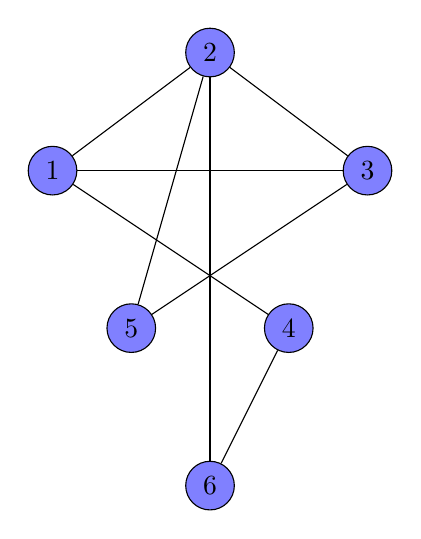
\begin{tikzpicture}
                % Nodes
                \node[circle, draw, fill=blue!50] (1) at (0, 0) {1};   % Internal node
                \node[circle, draw, fill=blue!50] (2) at (2, 1.5) {2}; % Internal node
                \node[circle, draw, fill=blue!50] (3) at (4, 0) {3}; % Leaf
                \node[circle, draw, fill=blue!50] (4) at (3, -2) {4}; % Leaf
                \node[circle, draw, fill=blue!50] (5) at (1, -2) {5}; % Leaf
                \node[circle, draw, fill=blue!50] (6) at (2, -4) {6}; % Leaf
                
                % Edges
                \draw (1) -- (2);
                \draw (1) -- (3);
                \draw (1) -- (4);
                \draw (2) -- (5);
                \draw (2) -- (3);
                \draw (2) -- (6);
                \draw (3) -- (5);
                \draw (4) -- (6);
            \end{tikzpicture}
        \end{minipage}
        \hfill
        \pause
        \begin{minipage}
            {0.45\textwidth}
            \centering
            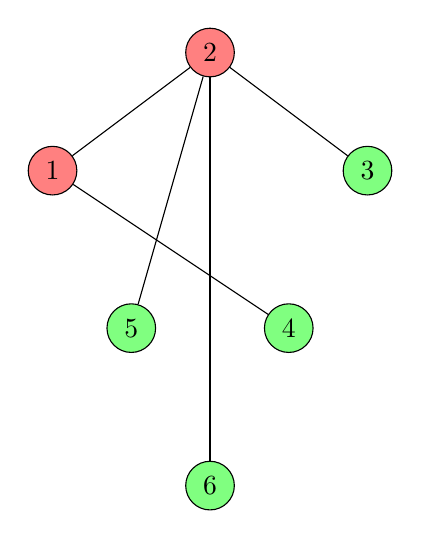
\begin{tikzpicture}
                % Nodes
                \node[circle, draw, fill=red!50] (1) at (0, 0) {1};   % Internal node
                \node[circle, draw, fill=red!50] (2) at (2, 1.5) {2}; % Internal node
                \node[circle, draw, fill=green!50] (3) at (4, 0) {3}; % Leaf
                \node[circle, draw, fill=green!50] (4) at (3, -2) {4}; % Leaf
                \node[circle, draw, fill=green!50] (5) at (1, -2) {5}; % Leaf
                \node[circle, draw, fill=green!50] (6) at (2, -4) {6}; % Leaf
                
                % Edges for spanning tree
                \draw (1) -- (2);
                \draw (1) -- (4);
                \draw (2) -- (5);
                \draw (2) -- (3);
                \draw (2) -- (6);
            \end{tikzpicture}
        \end{minipage}
        \vspace{15pt}
        \captionof{figure}{Maximum Leaf Spanning Tree}
    \end{frame}
    \begin{frame}{Problem Definition}
        The Maximum Leaf Spanning Tree (MaxLST) problem comes in two primary versions.
        \begin{enumerate}
            \item<2-> \textbf{Optimization Version:} \\In this version, the goal is to maximize the number of leaf nodes in the spanning tree of a given graph.
            \item<3-> \textbf{Decision Version:}\\The decision version of the MLST problem asks whether it is possible to find a spanning tree with at least a given number of leaf nodes.
        \end{enumerate}
    \end{frame}
    \begin{frame}{Optimization Version of MaxLST}
        \textbf{Problem Statement:}
        \begin{itemize}[<+->]
            \item \textbf{Input:} \par A connected, undirected graph $ G=(V,E) $, where $V$ is the set of vertices and $E$ is the set of edges.
            \item \textbf{Objective:} \par Find a spanning tree of $G$ that maximizes the number of leaf nodes 
        \end{itemize}
    \end{frame}
    \begin{frame}{Decision Version of MaxLST}
        \textbf{Problem Statement:}
        \begin{itemize}[<+->]
            \item \textbf{Input:} \par A connected, undirected graph $ G=(V,E) $, and an integer $k$.
            \item \textbf{Question:} \par Does there exist a spanning tree of $G$ with at least $k$ leaf nodes? 
        \end{itemize}
    \end{frame}
\end{section}

\begin{section}{Complexity Analysis of MaxLST}
    \begin{frame}{Complexity of MaxLST}
        \begin{description}[<+->]
            \item[The MaxLST problem], particularly the decision version of the problem is an NP-Complete problem. Which means that the problem is both in the NP and NP-Hard class of problems.
            \item[NP problems] or Nondeterministic Polynomial time problem is the set of all decision problems solvable in polynomial time by a non-deterministic algorithm. A problem is in NP if it's solution can be verified in polynomial time.
            \item[NP-Hard Problems] are the set of all those problems that are as hard as the hardest problem in NP. We prove a problem is NP-Hard by reducing an instance of a well known NP problem such as 3-SAT, Vertex Cover, Independent Set to an instance of the relevant problem
        \end{description}
    \end{frame}
    \begin{frame}{Proof: MaxLST is in NP}
        \begin{itemize}
            \setlength{\itemsep}{15pt}
            \item Given a solution $T$, for a Graph $G=(V,E)$ and a integer $k$ is given, we can just check if the tree has k leaves or more.
            \item By applying a simple BFS or DFS we can both check
            \begin{itemize}
                \setlength{\itemsep}{3pt}  
                \item[] -- if the solution is indeed a spanning tree.
                \item[] -- if it has k leaves.
            \end{itemize}
            \item So, the MaxLST problem is in NP
        \end{itemize}
    \end{frame}
    \begin{frame}{Proof: MaxLST is in NP-Hard}
        We prove the NP-hardness of Max-Leaf Spanning Tree in two steps -\\
        \begin{enumerate} [<+->]
            \setlength{\itemsep}{5pt}
            \item Reduce the Minimum Vertex Cover problem to Minimum Connected Dominating Set (MinCDS) problem.
            \item Show that Minimum Connected Dominating Set is equivalent to Max-Leaf Spanning Tree problem.
        \end{enumerate}
    \end{frame}
    \begin{frame}{Minimum Vertex Cover Problem}
        \begin{description}[<+->]
            \item[Vertex Cover:]Given a graph $G=(V,E)$, where $V$ is the set of vertices and $E$ is the set of edges, a vertex cover is a subset of vertices $C \subseteq V$ such that every edge in the graph has at least one of its endpoints in $C$. 
            \item[Objective:] We want a subset $C \subseteq V$ such that for every edge $(u,v) \in E$, at least one of the vertices $u$ or $v$ is in $C$, and the number of vertices in $C$ is minimized. 
            \item[Question:]Given a connected graph $G = (V, E)$ and an integer $k$, does $G$ have a vertex cover of size at most $k$?   
        \end{description}
    \end{frame}
    \begin{frame}{Example}
        \begin{columns}

    % First column (Graph with 6 Nodes)
            \begin{column}{0.45\textwidth}
                \centering
                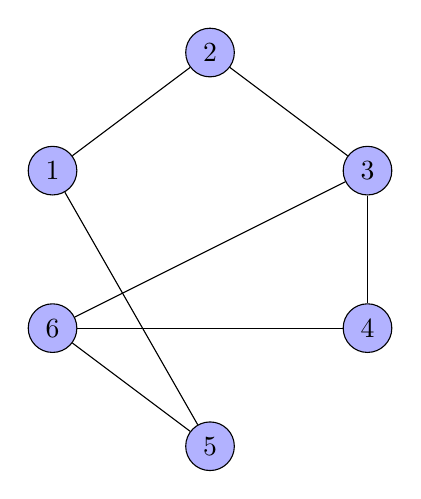
\begin{tikzpicture}
            
                    % Adjusted Node coordinates for better layout
                    \node[circle, draw, fill=blue!30] (1) at (0, 2) {1};   
                    \node[circle, draw, fill=blue!30] (2) at (2, 3.5) {2};  
                    \node[circle, draw, fill=blue!30] (3) at (4, 2) {3};   
                    \node[circle, draw, fill=blue!30] (4) at (4, 0) {4};  
                    \node[circle, draw, fill=blue!30] (5) at (2, -1.5) {5}; 
                    \node[circle, draw, fill=blue!30] (6) at (0, 0) {6};  
                    
                    % Edges
                    \draw (1) -- (2);
                    \draw (1) -- (5);
                    \draw (2) -- (3);
                    \draw (3) -- (4);
                    \draw (3) -- (6);
                    \draw (4) -- (6);
                    \draw (5) -- (6);
            
                \end{tikzpicture}
                \end{column}
            
                % Second column (Minimum Vertex Cover Highlighted)
                \begin{column}{0.45\textwidth}
                \centering
                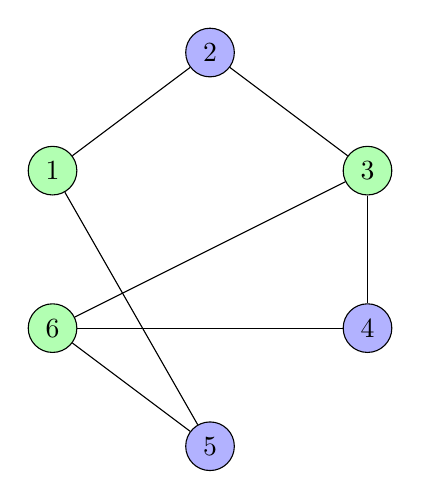
\begin{tikzpicture}
            
                    % Adjusted Node coordinates for better layout
                    \node[circle, draw, fill=green!30] (1) at (0, 2) {1};   
                    \node[circle, draw, fill=blue!30] (2) at (2, 3.5) {2};  
                    \node[circle, draw, fill=green!30] (3) at (4, 2) {3};   
                    \node[circle, draw, fill=blue!30] (4) at (4, 0) {4};  
                    \node[circle, draw, fill=blue!30] (5) at (2, -1.5) {5}; 
                    \node[circle, draw, fill=green!30] (6) at (0, 0) {6};  
                    
                    % Edges
                    \draw (1) -- (2);
                    \draw (1) -- (5);
                    \draw (2) -- (3);
                    \draw (3) -- (4);
                    \draw (3) -- (6);
                    \draw (4) -- (6);
                    \draw (5) -- (6);
            
                \end{tikzpicture}
            \end{column}
        \end{columns}
        \vspace{15pt}
        \captionof{figure}{Minimum Vertex cover in a graph}
    \end{frame}
    
    \begin{frame}{Minimum Connected Dominating Set Problem}
        \begin{description}[<+->]
            \item[Dominating Set:]Given a graph $G=(V,E)$, where $V$ is the set of vertices and $E$ is the set of edges, a dominating set is a subset of vertices $D \subseteq V $such that every vertex in the graph is either in $D$ or adjacent to a vertex in $D$. 
            \item[Objective:] We want a subset $D \subseteq V$ such that for every node $u \in V$, $u$ is either in $D$ or is adjacent to a node $v \in D$ , the nodes in $D$ create a connected sub-graph and the number of vertices in $D$ is minimized. 
            \item[Question:]Given a connected graph $G = (V, E)$ and an integer $k$, does $G$ have a connected dominating set of size at most $k$?  
        \end{description}
    \end{frame}
    \begin{frame}{Example}

        \begin{columns}
        
            % First column (first TikZ picture)
            \begin{column}{0.45\textwidth}
            \centering
            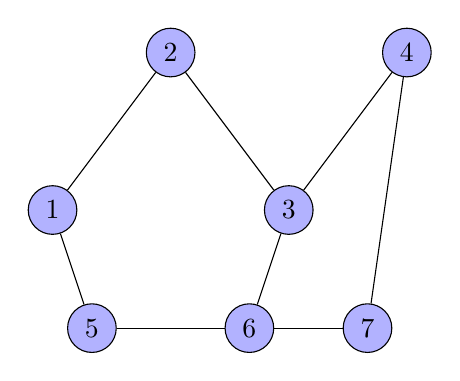
\begin{tikzpicture}
        
                % Nodes
                \node[circle, draw, fill=blue!30] (1) at (0, 0) {1};   
                \node[circle, draw, fill=blue!30] (2) at (1.5, 2) {2};  
                \node[circle, draw, fill=blue!30] (3) at (3, 0) {3};   
                \node[circle, draw, fill=blue!30] (4) at (4.5, 2) {4};  
                \node[circle, draw, fill=blue!30] (5) at (0.5, -1.5) {5}; 
                \node[circle, draw, fill=blue!30] (6) at (2.5, -1.5) {6};  
                \node[circle, draw, fill=blue!30] (7) at (4, -1.5) {7};  
                
                % Edges
                \draw (1) -- (2);
                \draw (1) -- (5);
                \draw (2) -- (3);
                \draw (3) -- (4);
                \draw (3) -- (6);
                \draw (4) -- (7);
                \draw (5) -- (6);
                \draw (6) -- (7);
        
            \end{tikzpicture}
            \end{column}
            % Second column (second TikZ picture)
            \begin{column}{0.45\textwidth}
            \centering
            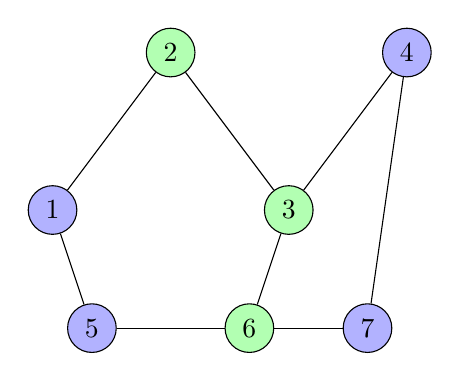
\begin{tikzpicture}
        
                % Nodes
                \node[circle, draw, fill=blue!30] (1) at (0, 0) {1};   
                \node[circle, draw, fill=green!30] (2) at (1.5, 2) {2};  
                \node[circle, draw, fill=green!30] (3) at (3, 0) {3};   
                \node[circle, draw, fill=blue!30] (4) at (4.5, 2) {4};  
                \node[circle, draw, fill=blue!30] (5) at (0.5, -1.5) {5}; 
                \node[circle, draw, fill=green!30] (6) at (2.5, -1.5) {6};  
                \node[circle, draw, fill=blue!30] (7) at (4, -1.5) {7};    
                
                % Edges
                \draw (1) -- (2);
                \draw (1) -- (5);
                \draw (2) -- (3);
                \draw (3) -- (4);
                \draw (3) -- (6);
                \draw (4) -- (7);
                \draw (5) -- (6);
                \draw (6) -- (7);
        
            \end{tikzpicture}
            \end{column}
        
        \end{columns}
        \vspace{15pt}
        \captionof{figure}{Minimum Connected Dominating Set in a graph}
    \end{frame}
    \begin{frame}{Reduction from VC to MinCDS}
        Given a vertex cover instance $G = (V, E)$, we reduce it to a minimum connected dominating set instance $G' = (V', E')$ as follows -
        \begin{itemize}
            \item $G'$ has the complete graph induced by V.
            \item for each edge $(u,v) \in E$ we add a node $x_{uv}$ in $V'$ and add two edges $(u,x_{uv})$ and $(v,x_{uv})$
        \end{itemize}
        Formally-
        \begin{exampleblock}{}
            \centering
            \[
                V' = V \cup \{ x_{uv} : (u,v) \in E\} \\
                E' = \{(u,v) : u \in V, v \in V~ and~ u \neq v \} \cup \{(x_{uv},u) : (u,v) \in E \}
            \]
            \vspace{15pt}
        \end{exampleblock}
        This is clearly reducible in polynomial time.
    \end{frame}
    \begin{frame}{Reduction from VC to MinCDS Example}
        \centering
        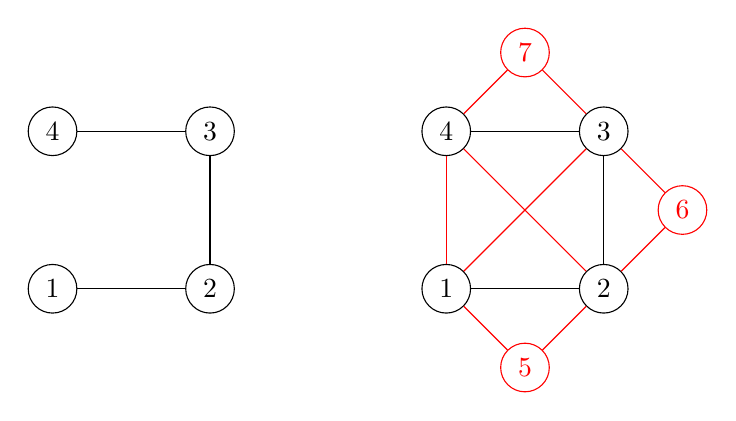
\begin{tikzpicture}
            % First Graph (Left)
            \node (A1) at (0, 0) [circle, draw] {1};
            \node (A2) at (2, 0) [circle, draw] {2};
            \node (A3) at (2, 2) [circle, draw] {3};
            \node (A4) at (0, 2) [circle, draw] {4};
            
            \draw (A1) -- (A2);
            \draw (A2) -- (A3);
            \draw (A3) -- (A4);
            
            % Second Graph (Right)
            \node (B1) at (5, 0) [circle, draw] {1};
            \node (B2) at (7, 0) [circle, draw] {2};
            \node (B3) at (7, 2) [circle, draw] {3};
            \node (B4) at (5, 2) [circle, draw] {4};
            
            % Red vertices
            \node (B5) at (6, -1) [circle, draw=red, text=red] {5};
            \node (B6) at (8, 1) [circle, draw=red, text=red] {6};
            \node (B7) at (6, 3) [circle, draw=red, text=red] {7};
            
            % Edges of the second graph
            \draw (B1) -- (B2);
            \draw (B2) -- (B3);
            \draw (B3) -- (B4);
            
            % Red edges
            \draw[red] (B5) -- (B1);
            \draw[red] (B5) -- (B2);
            \draw[red] (B6) -- (B2);
            \draw[red] (B6) -- (B3);
            \draw[red] (B7) -- (B3);
            \draw[red] (B7) -- (B4);
            \draw[red] (B1) -- (B3);
            \draw[red] (B2) -- (B4);
            \draw[red] (B1) -- (B4);
        \end{tikzpicture}
        \vspace{15pt}
        \captionof{figure}{Reduction from VC to MinCDS}
    \end{frame}
    \begin{frame}{Reduction from VC to MinCDS (cont.)}
        \begin{block}{Necessity} 
        Let $S$ be a vertex cover of $G$. For any $v \in V'$, there are two cases- 
            \begin{enumerate}
                \item $v \in V $: By the definition of vertex cover we know that $v$ is dominated by $S$
                \item $v=v_{xy}$ is an edge vertex: Because $(x,y)$ is covered by $S$, then $x \in S$ or $y \in S$, $v_{xy}$ is dominated by $S$ 
            \end{enumerate}
            Thus $S$ is a connected dominating set of $G'$
        \end{block}
    \end{frame}
    \begin{frame}{Reduction from VC to MinCDS (cont.)}
        \begin{block}{Sufficiency} 
        Let $S$ be a connected dominating set in $G'$. 
            \begin{itemize}
                \item We first observe that for any edge vertex $v_{xy}$ in, it can only be dominated by $x$ or $y$
                \item For any edge vertex $v_{xy} \in S$. The replacement does not increase the cardinality of $S$ and mantains $S$'s property of being a dominating set.
                \item Now $S$ contains no edge vertex, so every edge vertex is dominated by $S$, that is to say, every edge in $G$ has at least one endpoint in $S$
.
            \end{itemize}
            Thus $S$ is a vertex cover for $G$
        \end{block}
    \end{frame}
    \begin{frame}{Equivalence of MinCDS to MaxLST}
        \small
        \begin{block}{Proving Equivalence}
             A connected graph $G = (V, E)$ has a connected dominating set $S$ of size at most $k$ if and only if it has a spanning tree $T$ of at least $n - k$ leaves.
        \end{block}
        \pause
        \begin{block}{Necessity}
             Let $T$ be a spanning tree of the sub-graph induced by $S$. For each vertex $v \in V \backslash S$, there exists a vertex $u \in S$ where $(u,v) \in E$. We add these vertices $u$ and the edges $(u, v)$ to $T$. All newly added nodes are new in $T$, has a degree of 1 and doesn't add a cycle. That is, $T$ is still a spanning tree. Therefore, $|Leaves(T)| \geq n - k$
        \end{block}
        \pause
        \begin{block}{Sufficiency}
            Let $T$ be a spanning tree of $V$ with at least $n-k$ leaves. Every leaf $v$ is dominated by an inner vertex and all inner vertices are connected. So they form a dominating set $S$ and $|S| \leq k$.
        \end{block}
    \end{frame}
\end{section}
\begin{section}{Existing Algorithms}
    \begin{subsection}{Exact Exponential Algorithms}
        \begin{frame}{Exact Algorithms}
\begin{center}
    \textbf{\textcolor{blue}{Table:} Exact Exponential Algorithms}
\end{center}

\centering
\scriptsize
\begin{tabular}{m{2.5cm}m{1.75cm}m{0.75cm}m{1.9cm}m{2.3cm}}
\hline
\textbf{Algorithm}           & \textbf{Runtime}                & \textbf{Year} & \textbf{Author}                                & \textbf{Comment}                                            \\ \hline
Naive brute-force & $\Omega(2^n)$ & - & - & Considering all possible leafset \\ \hline
Simple Branching \cite{Kneis2008ANA}     & $O(4^kpoly(n))$           & 2008          & Kneis, Langer, and Rossmanith                  & Parameterized in the number of leaves $k$                   \\ \hline
Improved Branching \cite{daligault2010fpt}   & $O(3.72^kpoly(n))$        & 2010          & Daligault et al.                               & Parameterized in the number of leaves $k$                   \\ \hline
Connected Dom Set \cite{fomin2008solving}    & $O(1.9407^n)$                   & 2008          & Fomin, Grandoni, and Kratsch                   & Equivalent to MaxLST                                        \\ \hline
Branching Algo \cite{fernau2011exact}       & $O(1.8966^n)$                   & 2011          & Fernau et al.                                  & Branching algo based on some properties                     \\ \hline
Worst Case Lower Bound \cite{fernau2011exact} & $\Omega(1.4422^n)$              & -             & -                                              & Lower Bound                                                 \\ \hline
\end{tabular}
\end{frame}


        \begin{frame}{Branching Algorithm}
            \begin{itemize}
                \item Proposed by Fernau et. al at IWPEC 2009
                \item Improves upon the previous approach where leaves of a subtree of the graph were repeatedly branched in order to decide whether it can remain a leaf or must become an internal node of the spanning tree. (Kneis et.al and Dalgaut et. al)
                \item In that approach branching on nodes of small degree (with two possible successors) becomes the worst case resulting in a bad running time.
                \item Fernau et. al improved upon the technique by marking nodes as leaves as early as possible even when they are not yet attached to an internal node.
                \item The algorithm maintains 5 disjoint sets of vertices to mark the nodes and terminates when it has found a spanning tree
            \end{itemize}
        \end{frame}
        \begin{frame}{Node Sets Definition}
            \begin{description}[<+->]
                \item[Internal Nodes(IN):] The nodes that were decided to be internal nodes of the spanning tree.
                \item[Leaf Nodes(LN):]Nodes decided to be leaves in the spanning tree. All neighbors of these nodes are already processed
                \item[Branching Nodes(BN):] Nodes that are right now treated as leaves but all their neighbors haven't been processed i.e they are candidates for branching.  
            \end{description}
            \centering
            \only<4>{
                \includegraphics[width=0.75\textwidth]{IN,LN,BN.png}
            }
        \end{frame}
        \begin{frame}{Node Sets Definition(cont.)}
            \begin{description}[<+->]
                \item[Floating Leaves(FL):] The nodes that were decided to be leaves of the spanning tree but hasn't been attached to the current spanning tree yet.
                \item[Free Nodes(FN):] All the rest of the nodes that haven't been attached to the tree and hasn't been decided as leaves either. 
            \end{description}
            \centering
            \only<3>{
                \includegraphics[width=0.5\textwidth]{FL,FN.png}
                \captionof{figure}{Free Nodes (in white) and Floating Leaves (in red)}
            }
        \end{frame}
        \begin{frame}{Reduction Rules}
            The algorithm applies the following reduction rules recursively to reduce the search space-
            \begin{enumerate}[<+->]
                \item If there exist two adjacent vertices $u, v \in V$ such that $u, v \in FL$ or $u, v \in BN$, then remove the edge $(u, v)$ from $G$.
                \item  If there exists a node $v \in BN$ with $d(v) = 0$, then move $v$ into $LN$
                \item If there exists a free vertex $v$ with $d(v) = 1$, then move $v$ into $FL$.
                \item  If there exists a free vertex $v$ with no neighbors in $Free \cup FL$, then move $v$ into $FL$
                \item If there exists a triangle $\{x, y, z\}$ in $G$ with $x$ a free vertex and $d(x) = 2$, then move $x$ into $FL$.
                \item If there exists a node $u \in BN$ which is a cut vertex in $G$, then move $u$ into $IN$.
                \item If there exist two adjacent vertices $u, v \in V$ such that $u \in LN$ and $v \in V \backslash IN$, then remove the edge $(u, v)$ from G.
            \end{enumerate}
        \end{frame}
        \begin{frame}{Branching and Halting Rules}
                \small
                \textcolor{mqdeepred}{\textbf{\large Branching Rules:}}
                \begin{enumerate}[<+->]
                    \item if $d(v) \geq 3$ or if $d(v) = 2$ and none of $v$'s neighbours are in FL then branch into two solutions where $v$ is in IN or in LN 
                    \item if $d(v)=2$,  branches based on the degrees of its neighbors $\{x_1,x_2\}$, deciding whether $v$ and its neighbors should be leaves or internal nodes
                    \item if $d(v)=1$, the algorithm extends a path from $v$ and branches based on its final neighbor, deciding whether vertices along the path become leaves or internal nodes.
                    \item whenever a node $v$ becomes an internal node, all it's neighbors are attached to the tree as well.
                    \item Over the course of the algorithm only nodes in BN or Free can change sets. Other nodes must remain in their sets.
                \end{enumerate}
                \only<6->{\textcolor{mqdeepred}{\textbf{\large Halting Rules:}}}
                \begin{enumerate}[<+->]
                    \item If at any point a node is found as unreachable after reduction, we return 0 denoting a failure
                    \item if all nodes are either in IN or LN we return size of LN as answer. 
                \end{enumerate}
        \end{frame}
    \end{subsection}
    \begin{subsection}{Approximation Algorithms}
        \begin{frame}{Existing Approximation Algorithms}
            \begin{center}
    \textbf{\textcolor{blue}{Table:} Approximation Algorithms}
\end{center}

\centering
\scriptsize
\begin{tabular}{m{2.5cm}m{1.5cm}m{1.25cm}m{1.75cm}m{2.3cm}}
\hline
\textbf{Algorithm}           & \textbf{Complexity}                & \textbf{Approx ratio} & \textbf{Author}                                & \textbf{Comment}                                            \\ \hline
Local Optimization\cite{lu1996power} & $O(n^4)$ &  Approx. 5 &  Lu and Ravi &  Local Approximation Technique \\ \hline
 Local Optimization \cite{lu1996power}     & $O(n^7)$           &  Approx. 3          &  Lu and Ravi                  &  Local Approximation Technique                  \\ \hline
Greedy \cite{LU1998132}   & $ O((m+n)\alpha(m,n))$        &  Approx. 3          &  Lu and Ravi                               &  Introduced Leafy Forests                  \\ \hline
 Incrementally building a subgraph \cite{solis20172}    & $O(m)$                   &  Approx. 2          & Solis-Oba, Bonsma, and Lowski                   &  Uses expansions rule                                        \\ \hline
Expands the tree       & $O(m)$                   &  Approx. 2          & Liao and Lu                                  &  Simple, Year2023        \\ \hline
                                               
\end{tabular}
        \end{frame}
        \begin{frame}{Incremental Sub-graph Construction}
            \begin{itemize}
                \item Introduced by Roberto Solis-Oba at ESA 1998 
                \item The first constant factor approximation algorithm was developed by Lu and Ravi with an approximation ratio of 3 and 5\cite{lu1996power}. They later introduced the idea of leafy forests to create a more efficient algorithm\cite{LU1998132}.
                \item Solis-soba et. al introduced prioritized expansion rules to improve the approximation ratio to 2 for graphs with maximum degree of at least 3. 
                \item The priority of a rule reflects the number of leaves that the rule adds to the forest. Hence it is desirable to use only ‘high’ priority rules to build the forest.
                \item The ‘low’ priority rules are needed though to ensure that the number of components of the forest can be kept small enough.
            \end{itemize}
        \end{frame}
        \begin{frame}{Notations}
            \begin{itemize}
                \item $V(G) \RightArrow$ Set of all nodes of $G$.
                \item $\overline{V(G)} \RightArrow$ Set of all nodes not in $G$.
                \item $L(G) \RightArrow$ Set of leaves of $G$.
                \item $N_G(v) \RightArrow$ Neighborhood of node $v$ in $G$.
            \end{itemize}
            \begin{block}{Expanding a node $v$}
                Let $F$ be a a (possibly empty) subgraph of a graph $G$. The operation of expanding a vertex $v \in V(G)$ consists of -
                \begin{itemize}
                    \item[] -- Adding $v$ to $F$, in case $v \notin V(F)$
                    \item[] -- For every $w \in N_G(v) \backslash V(F)$: adding vertex $w$ and edge $(v,w)$ to $F$
                \end{itemize}
                This operation yields a new subgraph $F'$ of $G$ which is a forest if F was a forest and if $v \notin V(F)$ it increases the number of components of F by 1
            \end{block}
        \end{frame}
        \begin{frame}{Expansion Rules}
            We use the following four expansion rules, where the given order defines the priorities. That is, if for any node Rule 2 can be applied, then Rule 3 or 4 can't be applied.
            \begin{enumerate}
                \item If $F$ contains a vertex $v$ with at least two neighbors in $\overline{V(F)}$, then expand $v$.
                \item  If $F$ contains a vertex $v$ with only one neighbor $w$ in $\overline{V(F)}$, which in turn has at least three neighbors in $\overline{V(F)}$, then first expand $v$, and next expand $w$.
                \item If $F$ contains a vertex $v$ with only one neighbor $w$ in $\overline{V(F)}$, which in turn has two neighbors in $\overline{V(F)}$, then first expand $v$, and next expand $w$.
                \item If$\overline{V(F)}$ contains a vertex $v$ with at least three neighbors in $\overline{V(F)}$, then expand $v$.
            \end{enumerate}
        \end{frame}
        \begin{frame}{Expansion Rules(cont.)}
            \centering
            \includegraphics[height=3.5cm]{solis.png}
            \\
            \raggedright
            As we can see that, only rule 4 can increase the number of components. As this rule has the least priority, we limit the number of components. Also, once a new component has been introduced no other rule can change this as they don't operate on nodes already in the forest.\\
            Since G has a maximum degree of at least 3, Rule 4 also ensures that the resulting forest is never empty. 
        \end{frame} 
        \begin{frame}{Algorithm}
            \begin{enumerate}
                \item We start with an empty forest $F$
                \item Apply the expansion rules 1-4 as long as one of them can be applied on some node
                \item We randomly choose a vertex in $F$ and expanding it until we obtain a spanning subgraph.
                \item Arbitrary edges are added to $F$ without creating cycles, until a connected spanning tree is not obtained
                \item This is the solution tree for MaxLST
            \end{enumerate}
        \end{frame}
    \end{subsection}
    \begin{subsection}{Heuristic And Meta-heuristic Algorithms}
        \begin{frame}{Heuristic And Meta-heuristic Algorithms}
            \textcolor{mqdeepred}{\textbf{\large Heuristic Algorithms:}}
            \begin{itemize}
                \item BFS Algorithm
                \item Priority BFS
                \item Max Priority BFS
            \end{itemize}
            \textcolor{mqdeepred}{\textbf{\large Meta-Heuristic Algorithms:}}
            \begin{itemize}
                \item Simulated Annealing
                \item Genetic Algorithm
                \item Artificial Bee Colony Algorithm
            \end{itemize}
        \end{frame}
        \begin{frame}{Comparison between Heuristic And Meta-heuristic Algorithms}
            \begin{figure}
                \centering
                \includegraphics[width=\linewidth]{exp.png}
                \caption{Experiments on small complete grid graphs\cite{bruggemanndevelopment}}
                \label{fig:enter-label}
            \end{figure}
        \end{frame}
        \begin{frame}{Comparison between Heuristic And Meta-heuristic Algorithms}
            \begin{figure}
                \centering
                \includegraphics[width=\linewidth]{Screenshot_20241020_034159.png}
                \caption{Experiments on small random graphs\cite{bruggemanndevelopment}}
                \label{fig:enter-label}
            \end{figure}
        \end{frame}
    \end{subsection}
\end{section}

\begin{section}{Experiments}
    \begin{frame}{Experiments}
        We will be comparing the performance of our chosen algorithms with the following algorithms -
        \begin{itemize}
            \item BFS
            \item Max Priority BFS
            \item Artificial Bee Colony Algorithm
            \item Genetic Algorithm
        \end{itemize}
        The comparisons will be done in these types of dense and sparse graphs-
        \begin{itemize}
            \item Random Graph
            \item D-regular graph
            \item Complete and Incomplete Grid graphs
        \end{itemize}
    \end{frame}
\end{section}

\begin{section}{Applications}
    \begin{subsection}{Theoretical Applications}
        \begin{frame}{Phylogenetic Tree}
\begin{columns}

    % First column (50% width for the image)
    \begin{column}{0.5\textwidth}
        \centering
        \includegraphics[height=5cm]{pgtreer.png} % Add the correct file name of your image
        \end{column}
    
        % Second column (50% width for the text)
        \begin{column}{0.5\textwidth}
    Phylogenetic trees are designed to increase species representation while minimizing internal nodes. MLST contributes to this by identifying spanning trees with the greatest number of leaves, reflecting genuine species, and minimizing inferred shared ancestors. \newline \newline
    This is important for taxonomy and evolutionary studies because it allows researchers to focus on actual species rather than hypothetical ancestors.
    
    
    
    
    
        \end{column}
    
    \end{columns}
        
    \end{frame}
        \begin{frame}{More Theoretical Applications}
            \begin{itemize}
          \item \textbf{Clustering:}\newline  MLST can be used as a clustering algorithm, where each cluster is represented by a node in the spanning tree. The minimum latency ensures that clusters are closely related.\cite{gupta2003simpler}
          \newline
          \item \textbf{QoS Provisioning: }\newline
          Ensuring that quality of service (QoS) requirements are met for different applications.\cite{swamy2004primal}
        \end{itemize}
        \end{frame}
    \end{subsection}
    \begin{subsection}{Practical Applications}
    \begin{frame}{Ditributed Systems}
    
            \begin{columns}
            
                % First column (30% width for the image)
                \begin{column}{0.5\textwidth}
                    \centering
                    \includegraphics[width=\textwidth]{wns.png} % Add the correct file name of your image
                \end{column}
            
                % Second column (70% width for the text)
                \begin{column}{0.5\textwidth}
            
                By maximizing leaves, internal nodes are minimized. This is crucial in distributed systems where internal nodes represent servers or resources responsible for routing or control. Minimizing such nodes reduces complexity and resource consumption.\newline \newline
                This leads to more efficient communication and control protocols.\cite{PAYAN1984267}
            
                \end{column}
            
            \end{columns}

        \end{frame}
        \begin{frame}{Forest Fire management}
\begin{columns}

    % First column (50% width for the image)
    \begin{column}{0.5\textwidth}
        \centering
        \includegraphics[height=2cm]{fire.png} % Add the correct file name of your image
        \end{column}    
        % Second column (50% width for the text)
        \begin{column}{0.5\textwidth}
        MLST (Maximum Leaves Spanning Tree) helps optimize forest fire management by maximizing monitoring coverage and communication efficiency with minimal resources. It can improve sensor network design, firefighting coordination, and resource allocation, ensuring better preparedness and response to forest fires.\cite{hosseinmardi2023new}
    
    
    
    
    
        \end{column}
    
    \end{columns}
     
\end{frame}
    
    \begin{frame}{More Practical Applications}
        \begin{itemize}
      \item \textbf{Routing Protocols for Wireless Networks:}\newline In wireless networks, MLST can be used to determine the optimal topology for a mesh network. The network can achieve maximum throughput and minimize interference by selecting the links with the lowest latency.\cite{kamei2013self}\cite{guha1998approximation}\cite{schwartges2011approximation}
      \newline
      \item \textbf{Circuit Layouts:}\newline
      MLST can optimize circuit layout by minimizing wire length and delay. It helps identify the critical path for circuit optimization.\cite{storer1981constructing}
    \end{itemize}
    \end{frame}
    \end{subsection}
\end{section}





\begin{section}{Bibliography}
\begin{frame}[allowframebreaks]{References}
  \printbibliography  
\end{frame}
\end{section}


\end{document}